\documentclass[tikz,border=2pt]{standalone}
\usepackage{amsmath}
\usepackage{pgfplots}
\pgfplotsset{compat=1.18}
\usetikzlibrary{arrows.meta}
\begin{document}
% The three outcomes for max Z=x1+x2 with x>=0 and one constraint (Exercises 4.10, 4.11):
% x1+x2<=-1 is infeasible (s=1, t=-1 in Ex. 4.11); -x1+x2<=1 is unbounded along (lambda,0) (s=-1, t=1 in Ex. 4.10);
% x1+2x2<=1 has the triangle (0,0),(1,0),(0,1/2) and the unique optimum (1,0), Z=1 (s=1, t=2 in Ex. 4.10).
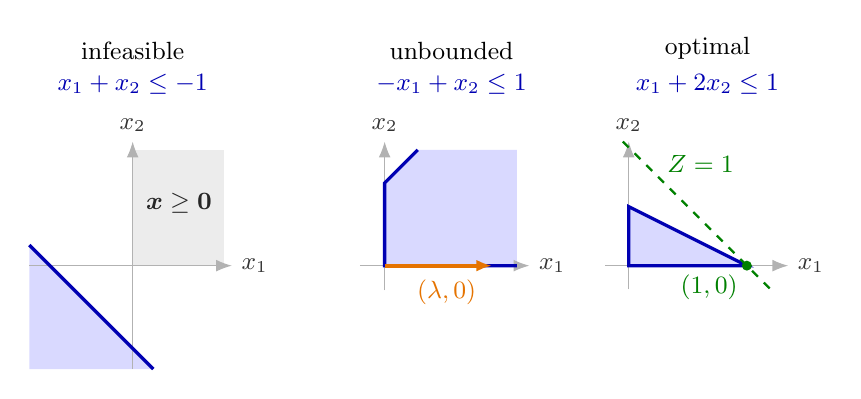
\begin{tikzpicture}[font=\small, >={Latex[length=2mm]}]
  % ---------------- infeasible ----------------
  \begin{scope}[x=1.05cm, y=1.05cm]
    \fill[gray!15] (0,0) rectangle (1.1,1.4);
    \fill[blue!15] (-1.25,0.25) -- (0.25,-1.25) -- (-1.25,-1.25) -- cycle;
    \draw[gray!60, ->] (-1.25,0) -- (1.2,0) node[anchor=west, gray!40!black] {$x_1$};
    \draw[gray!60, ->] (0,-1.25) -- (0,1.5) node[anchor=south, gray!40!black] {$x_2$};
    \draw[blue!70!black, very thick] (-1.25,0.25) -- (0.25,-1.25);
    \node[gray!30!black] at (0.56,0.75) {$\boldsymbol{x}\geq\boldsymbol{0}$};
  \end{scope}
  \node[anchor=south] at (0,2.5) {infeasible};
  \node[anchor=south, blue!70!black] at (0,2.05) {$x_1+x_2\leq-1$};
  % ---------------- unbounded ----------------
  \begin{scope}[xshift=3.2cm, x=1.05cm, y=1.05cm]
    \fill[blue!15] (0,0) -- (1.6,0) -- (1.6,1.4) -- (0.4,1.4) -- (0,1) -- cycle;
    \draw[gray!60, ->] (-0.3,0) -- (1.75,0) node[anchor=west, gray!40!black] {$x_1$};
    \draw[gray!60, ->] (0,-0.3) -- (0,1.5) node[anchor=south, gray!40!black] {$x_2$};
    \draw[blue!70!black, very thick] (1.6,0) -- (0,0) -- (0,1) -- (0.4,1.4);
    \draw[orange!90!black, line width=1.4pt, ->] (0,0) -- (1.3,0);
    \node[orange!90!black, anchor=north] at (0.75,-0.05) {$(\lambda,0)$};
  \end{scope}
  \node[anchor=south] at (4.05,2.5) {unbounded};
  \node[anchor=south, blue!70!black] at (4.05,2.05) {$-x_1+x_2\leq1$};
  % ---------------- optimal ----------------
  \begin{scope}[xshift=6.3cm, x=1.5cm, y=1.5cm]
    \fill[blue!15] (0,0) -- (1,0) -- (0,0.5) -- cycle;
    \draw[gray!60, ->] (-0.2,0) -- (1.35,0) node[anchor=west, gray!40!black] {$x_1$};
    \draw[gray!60, ->] (0,-0.2) -- (0,1.05) node[anchor=south, gray!40!black] {$x_2$};
    \draw[blue!70!black, very thick] (0,0) -- (1,0) -- (0,0.5) -- cycle;
    \draw[green!50!black, thick, dashed] (-0.05,1.05) -- (1.2,-0.2);
    \node[green!50!black, anchor=south west, inner sep=1pt] at (0.3,0.76) {$Z=1$};
    \fill[green!50!black] (1,0) circle (1.8pt);
    \node[green!50!black, anchor=north east, inner sep=1pt] at (0.95,-0.05) {$(1,0)$};
  \end{scope}
  \node[anchor=south] at (7.3,2.5) {optimal};
  \node[anchor=south, blue!70!black] at (7.3,2.05) {$x_1+2x_2\leq1$};
\end{tikzpicture}
\end{document}
